\documentclass{ximera}

%\usepackage{todonotes}

\newcommand{\todo}{}

\usepackage{tkz-euclide}
\tikzset{>=stealth} %% cool arrow head
\tikzset{shorten <>/.style={ shorten >=#1, shorten <=#1 } } %% allows shorter vectors

\usepackage{tkz-tab}  %% sign charts
\usetikzlibrary{decorations.pathreplacing} 

\usetikzlibrary{backgrounds} %% for boxes around graphs
\usetikzlibrary{shapes,positioning}  %% Clouds and stars
\usetikzlibrary{matrix} %% for matrix
\usepgfplotslibrary{polar} %% for polar plots
\usetkzobj{all}
\usepackage[makeroom]{cancel} %% for strike outs
%\usepackage{mathtools} %% for pretty underbrace % Breaks Ximera
\usepackage{multicol}

\usepackage{polynom}



\usepackage[many]{tcolorbox}  %% for titled boxes
\newtcolorbox{xbox}[1]{%
    tikznode boxed title,
    enhanced,
    arc=0mm,
    interior style={white},
    attach boxed title to top center= {yshift=-\tcboxedtitleheight/2},
    fonttitle=\bfseries,
    colbacktitle=white,coltitle=black,
    boxed title style={size=normal,colframe=white,boxrule=0pt},
    title={#1}}


\usepackage{array}
\setlength{\extrarowheight}{+.1cm}   
\newdimen\digitwidth
\settowidth\digitwidth{9}
\def\divrule#1#2{
\noalign{\moveright#1\digitwidth
\vbox{\hrule width#2\digitwidth}}}





\newcommand{\RR}{\mathbb R}
\newcommand{\R}{\mathbb R}
\newcommand{\N}{\mathbb N}
\newcommand{\Z}{\mathbb Z}

%\renewcommand{\d}{\,d\!}
\renewcommand{\d}{\mathop{}\!d}
\newcommand{\dd}[2][]{\frac{\d #1}{\d #2}}
\newcommand{\pp}[2][]{\frac{\partial #1}{\partial #2}}
\renewcommand{\l}{\ell}
\newcommand{\ddx}{\frac{d}{\d x}}
\newcommand{\ddt}{\frac{d}{\d t}}

\newcommand{\zeroOverZero}{\ensuremath{\boldsymbol{\tfrac{0}{0}}}}
\newcommand{\inftyOverInfty}{\ensuremath{\boldsymbol{\tfrac{\infty}{\infty}}}}
\newcommand{\zeroOverInfty}{\ensuremath{\boldsymbol{\tfrac{0}{\infty}}}}
\newcommand{\zeroTimesInfty}{\ensuremath{\small\boldsymbol{0\cdot \infty}}}
\newcommand{\inftyMinusInfty}{\ensuremath{\small\boldsymbol{\infty - \infty}}}
\newcommand{\oneToInfty}{\ensuremath{\boldsymbol{1^\infty}}}
\newcommand{\zeroToZero}{\ensuremath{\boldsymbol{0^0}}}
\newcommand{\inftyToZero}{\ensuremath{\boldsymbol{\infty^0}}}



\newcommand{\numOverZero}{\ensuremath{\boldsymbol{\tfrac{\#}{0}}}}
\newcommand{\dfn}{\textbf}
%\newcommand{\unit}{\,\mathrm}
\newcommand{\unit}{\mathop{}\!\mathrm}
\newcommand{\eval}[1]{\bigg[ #1 \bigg]}
\newcommand{\seq}[1]{\left( #1 \right)}
\renewcommand{\epsilon}{\varepsilon}
\renewcommand{\iff}{\Leftrightarrow}

\DeclareMathOperator{\arccot}{arccot}
\DeclareMathOperator{\arcsec}{arcsec}
\DeclareMathOperator{\arccsc}{arccsc}
\DeclareMathOperator{\si}{Si}
\DeclareMathOperator{\proj}{proj}
\DeclareMathOperator{\scal}{scal}


\newcommand{\tightoverset}[2]{% for arrow vec
  \mathop{#2}\limits^{\vbox to -.5ex{\kern-0.75ex\hbox{$#1$}\vss}}}
\newcommand{\arrowvec}[1]{\tightoverset{\scriptstyle\rightharpoonup}{#1}}
\renewcommand{\vec}{\mathbf}
\newcommand{\veci}{\vec{i}}
\newcommand{\vecj}{\vec{j}}
\newcommand{\veck}{\vec{k}}
\newcommand{\vecl}{\boldsymbol{\l}}

\newcommand{\dotp}{\bullet}
\newcommand{\cross}{\boldsymbol\times}
\newcommand{\grad}{\boldsymbol\nabla}
\newcommand{\divergence}{\grad\dotp}
\newcommand{\curl}{\grad\cross}
%\DeclareMathOperator{\divergence}{divergence}
%\DeclareMathOperator{\curl}[1]{\grad\cross #1}


\colorlet{textColor}{black} 
\colorlet{background}{white}
\colorlet{penColor}{blue!50!black} % Color of a curve in a plot
\colorlet{penColor2}{red!50!black}% Color of a curve in a plot
\colorlet{penColor3}{red!50!blue} % Color of a curve in a plot
\colorlet{penColor4}{green!50!black} % Color of a curve in a plot
\colorlet{penColor5}{orange!80!black} % Color of a curve in a plot
\colorlet{fill1}{penColor!20} % Color of fill in a plot
\colorlet{fill2}{penColor2!20} % Color of fill in a plot
\colorlet{fillp}{fill1} % Color of positive area
\colorlet{filln}{penColor2!20} % Color of negative area
\colorlet{fill3}{penColor3!20} % Fill
\colorlet{fill4}{penColor4!20} % Fill
\colorlet{fill5}{penColor5!20} % Fill
\colorlet{gridColor}{gray!50} % Color of grid in a plot

\newcommand{\surfaceColor}{violet}
\newcommand{\surfaceColorTwo}{redyellow}
\newcommand{\sliceColor}{greenyellow}




\pgfmathdeclarefunction{gauss}{2}{% gives gaussian
  \pgfmathparse{1/(#2*sqrt(2*pi))*exp(-((x-#1)^2)/(2*#2^2))}%
}


%%%%%%%%%%%%%
%% Vectors
%%%%%%%%%%%%%

%% Simple horiz vectors
\renewcommand{\vector}[1]{\left\langle #1\right\rangle}


%% %% Complex Horiz Vectors with angle brackets
%% \makeatletter
%% \renewcommand{\vector}[2][ , ]{\left\langle%
%%   \def\nextitem{\def\nextitem{#1}}%
%%   \@for \el:=#2\do{\nextitem\el}\right\rangle%
%% }
%% \makeatother

%% %% Vertical Vectors
%% \def\vector#1{\begin{bmatrix}\vecListA#1,,\end{bmatrix}}
%% \def\vecListA#1,{\if,#1,\else #1\cr \expandafter \vecListA \fi}

%%%%%%%%%%%%%
%% End of vectors
%%%%%%%%%%%%%

%\newcommand{\fullwidth}{}
%\newcommand{\normalwidth}{}



%% makes a snazzy t-chart for evaluating functions
%\newenvironment{tchart}{\rowcolors{2}{}{background!90!textColor}\array}{\endarray}

%%This is to help with formatting on future title pages.
\newenvironment{sectionOutcomes}{}{} 



%% Flowchart stuff
%\tikzstyle{startstop} = [rectangle, rounded corners, minimum width=3cm, minimum height=1cm,text centered, draw=black]
%\tikzstyle{question} = [rectangle, minimum width=3cm, minimum height=1cm, text centered, draw=black]
%\tikzstyle{decision} = [trapezium, trapezium left angle=70, trapezium right angle=110, minimum width=3cm, minimum height=1cm, text centered, draw=black]
%\tikzstyle{question} = [rectangle, rounded corners, minimum width=3cm, minimum height=1cm,text centered, draw=black]
%\tikzstyle{process} = [rectangle, minimum width=3cm, minimum height=1cm, text centered, draw=black]
%\tikzstyle{decision} = [trapezium, trapezium left angle=70, trapezium right angle=110, minimum width=3cm, minimum height=1cm, text centered, draw=black]


\title[Dig-In:]{Vertical asymptotes}

\outcome{Recognize when a limit is indicating there is a vertical asymptote.}
\outcome{Evaluate the limit as $x$ approaches a point where there is a vertical asymptote.}
\outcome{Match graphs of functions with their equations based on vertical asymptotes.}
\outcome{Discuss what it means for a limit to equal $\infty$.}
\outcome{Define a vertical asymptote.}
\outcome{Understand the relationship between limits and vertical asymptotes.}
\outcome{Find vertical asymptotes of famous functions.}
\outcome{Find vertical asymptotes by looking at a graph.}


\begin{document}
\begin{abstract}
We explore functions that ``shoot to infinity'' at certain points in
their domain.
\end{abstract}
\maketitle

Consider the function
\[
f(x) = \frac{1}{(x+1)^2}.
\]
\begin{image}
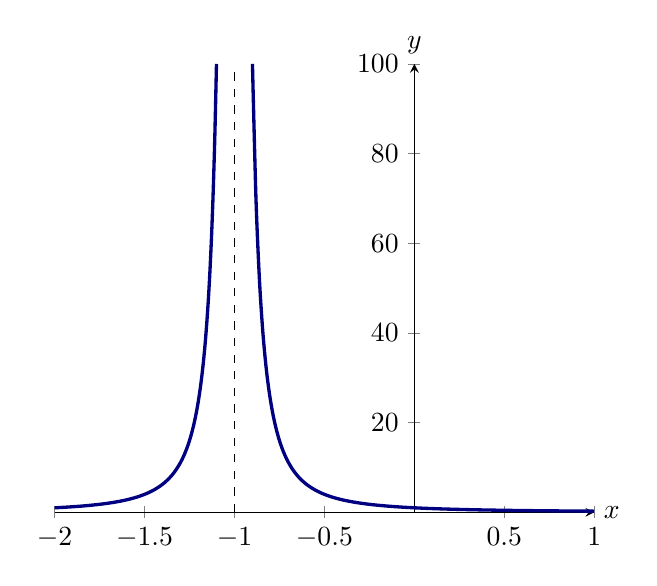
\begin{tikzpicture}
	\begin{axis}[
            domain=-2:1,
            ymax=100,
            samples=100,
            axis lines =middle, xlabel=$x$, ylabel=$y$,
            every axis y label/.style={at=(current axis.above origin),anchor=south},
            every axis x label/.style={at=(current axis.right of origin),anchor=west}
          ]
	  \addplot [very thick, penColor, smooth, domain=(-2:-1.1)] {1/(x+1)^2};
          \addplot [very thick, penColor, smooth, domain=(-.9:1)] {1/(x+1)^2};
          \addplot [textColor, dashed] plot coordinates {(-1,0) (-1,100)};
        \end{axis}
\end{tikzpicture}
%% \caption{A plot of $f(x)=\protect\frac{1}{(x+1)^2}$.}
%% \label{plot:1/(x+1)^2}
\end{image}
While the $\lim_{x\to -1} f(x)$ does not exist, something can still be
said.

\begin{definition}\label{def:inflimit}\index{limit!infinite}\index{infinite limit}
If $f(x)$ grows arbitrarily large as $x$ approaches $a$, we write
\[
\lim_{x\to a} f(x) = \infty
\]
and say that the limit of $f(x)$ \dfn{approaches infinity} as $x$
goes to $a$.

If $|f(x)|$ grows arbitrarily large as $x$ approaches $a$ and $f(x)$ is
negative, we write
\[
\lim_{x\to a} f(x) = -\infty
\]
and say that the limit of $f(x)$ \dfn{approaches negative infinity}
as $x$ goes to $a$.
\end{definition}

\begin{question}
  Which of the following are correct?
  \begin{selectAll}
    \choice[correct]{$\lim_{x\to -1} \frac{1}{(x+1)^2} = \infty$}
    \choice{$\lim_{x\to -1} \frac{1}{(x+1)^2} \to \infty$}
    \choice{$f(x) = \frac{1}{(x+1)^2}$, so $f(-1) = \infty$}
    \choice[correct]{$f(x) = \frac{1}{(x+1)^2}$, so as $x\to -1$,
      $f(x) \to \infty$}
  \end{selectAll}
\end{question}

On the other hand, consider the function 
\[
f(x) = \frac{1}{(x-1)}.
\]
\begin{image}
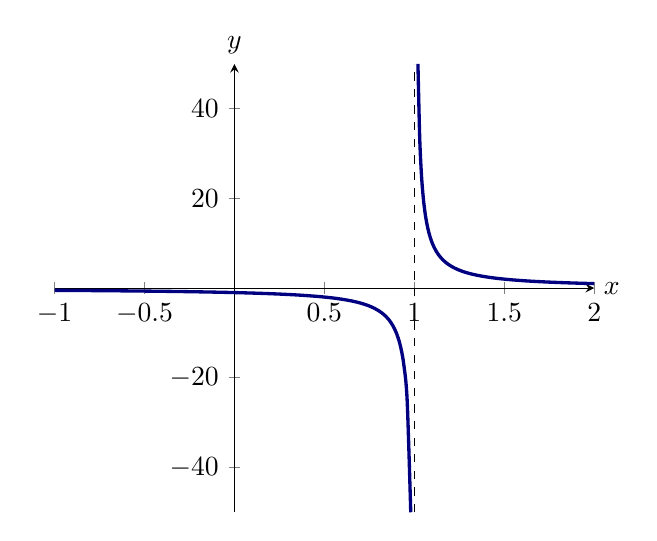
\begin{tikzpicture}
	\begin{axis}[
            domain=-1:2,
            ymax=50,
            ymin=-50,
            samples=100,
            axis lines =middle, xlabel=$x$, ylabel=$y$,
            every axis y label/.style={at=(current axis.above origin),anchor=south},
            every axis x label/.style={at=(current axis.right of origin),anchor=west}
          ]
	  \addplot [very thick, penColor, smooth, domain=(1.02:2)] {1/(x-1)};
          \addplot [very thick, penColor, smooth, domain=(-1:.98)] {1/(x-1)};
          \addplot [textColor, dashed] plot coordinates {(1,-50) (1,50)};
        \end{axis}
\end{tikzpicture}
%% \caption{A plot of $f(x)=\protect\frac{1}{x-1}$.}
%% \label{plot:1/(x-1)}
\end{image}
While the two sides of the limit as $x$ approaches $1$ do not agree, we can still consider the one-sided
limits.  We see $\lim_{x\to 1^+} f(x) = \infty$ and $\lim_{x\to 1^-} f(x) =
-\infty$.


\begin{definition}\label{def:vert asymptote}\index{asymptote!vertical}\index{vertical asymptote}
If at least one of the following hold:
\begin{itemize}
	\item $\lim_{x\to a} f(x) = \pm\infty$,
	\item $\lim_{x\to a^+} f(x) = \pm\infty$,
	\item $\lim_{x\to a^-} f(x) = \pm\infty$,
\end{itemize}
then the line $x=a$ is a \dfn{vertical asymptote} of $f$.
\end{definition}


\begin{example}
Find the vertical asymptotes of 
\[ f(x) = \frac{x^2-9x+14}{x^2-5x+6}. \]

\begin{explanation}
Start by factoring both the numerator and the denominator:
\[
\frac{x^2-9x+14}{x^2-5x+6} = \frac{(x-2)(x-7)}{(x-2)(x-3)}
\]
Using limits, we must investigate when $x\to 2$ and $x\to 3$. Write
\begin{align*}
\lim_{x\to 2} \frac{(x-2)(x-7)}{(x-2)(x-3)} &= \lim_{x\to 2} \frac{(x-7)}{(x-3)}\\
&= \frac{-5}{-1}\\
&=5.
\end{align*}
Now write
\begin{align*}
\lim_{x\to 3} \frac{(x-2)(x-7)}{(x-2)(x-3)} &= \lim_{x\to 3} \frac{(x-7)}{(x-3)}\\
&= \lim_{x\to 3}\frac{-4}{x-3}.
\end{align*}
Consider the one-sided limits separately.  Since $\lim_{x\to 3^+}
(x-3)$ approaches $0$ from the right and the numerator is negative,
$\lim_{x\to 3^+} f(x) = -\infty$. Since $\lim_{x\to 3^-} (x-3)$
approaches $0$ from the left and the numerator is negative,
$\lim_{x\to 3^-} f(x) = \infty$.
\begin{image}
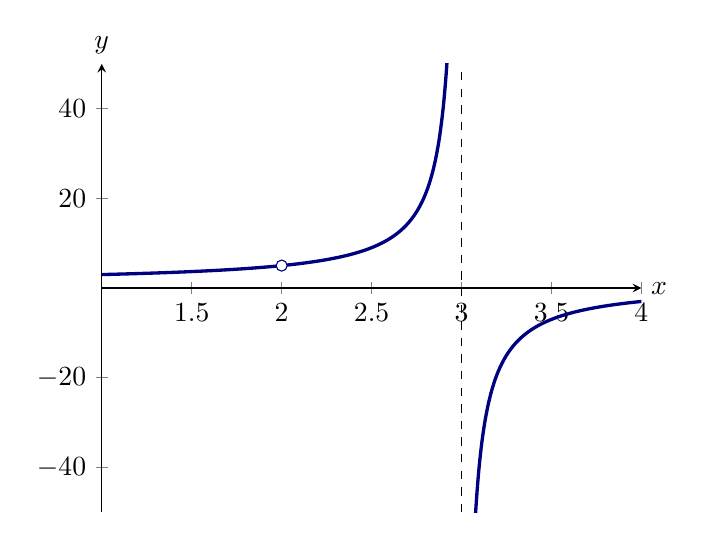
\begin{tikzpicture}
	\begin{axis}[
            domain=1:4,
            ymax=50,
            ymin=-50,
            samples=100,
            axis lines =middle, xlabel=$x$, ylabel=$y$,
            every axis y label/.style={at=(current axis.above origin),anchor=south},
            every axis x label/.style={at=(current axis.right of origin),anchor=west}
          ]
	  \addplot [very thick, penColor, smooth, domain=(3.02:4)] {(x-7)/(x-3)};
          \addplot [very thick, penColor, smooth, domain=(1:2.98)] {(x-7)/(x-3)};
          \addplot [textColor, dashed] plot coordinates {(3,-50) (3,50)};
          \addplot[color=penColor,fill=background,only marks,mark=*] coordinates{(2,5)};  %% open hole
        \end{axis}
\end{tikzpicture}
%% \caption{A plot of $f(x)=\protect\frac{x^2-9x+14}{x^2-5+6}$.}
%% \label{plot:(x^2-9x+14)/(x^2-5x+6)}
\end{image}
Hence we have a vertical asymptote at $x=3$.
\end{explanation}
\end{example}



\end{document}
